\documentclass[12pt,letterpaper]{article}

\usepackage[margin=1in]{geometry}
\usepackage{parskip}
\usepackage{booktabs}
\usepackage{enumitem}
\usepackage{tikz}
\usetikzlibrary{positioning,arrows.meta}
\usepackage[colorlinks=true,linkcolor=black,urlcolor=blue]{hyperref}

\title{Technical Report on the Migration of \texttt{chess.bc.ca} to a Git
Content Management System}
\author{British Columbia Chess Federation}
\date{July 2026}

\begin{document}

\maketitle

\section*{Executive Summary}

In July 2026 the British Columbia Chess Federation's website,
\url{https://chess.bc.ca}, was rebuilt from the ground up and moved to a new
hosting arrangement. Visitors see a modernized version of the same site ---
news, clubs, events, bulletins, champions, and so on --- but behind the
scenes everything has changed.

The old site was a collection of hand-edited web pages on a commercial web
server, costing about \$150 per year. Updating it required editing raw
HTML/PHP code and uploading files to the server, so in practice only one
person could maintain it.

The new site works differently:

\begin{itemize}[nosep]
  \item \textbf{It costs nothing to host.} The site is served by Netlify's
        free tier, eliminating the roughly \$150/year hosting fee. The only
        remaining cost is the annual domain-name registration for
        \texttt{chess.bc.ca}.
  \item \textbf{Anyone authorized can edit it.} Editors log into a simple
        web form at \url{https://chess.bc.ca/admin/} --- no coding
        knowledge, no special software. Posting a news item is as easy as
        filling out a form and clicking \emph{Publish}.
  \item \textbf{It looks good on phones.} The layout automatically adapts
        to any screen size.
  \item \textbf{It largely runs itself.} News items automatically move to
        the archive when they expire, the site rebuilds itself every night,
        and every change ever made is permanently recorded and reversible.
\end{itemize}

This report is written for the person who will maintain the site. It assumes
familiarity with basic web technologies and GitHub, but not with the other
tools involved. It explains what each piece of the system does, how the
pieces fit together, and how to perform routine maintenance.

\newpage
\tableofcontents
\newpage

\section{Introduction}

The previous \texttt{chess.bc.ca} was a PHP website: each time a visitor
requested a page, a program on the web server assembled the page from
fragments of PHP and HTML. There was no database and no administrative
interface; all changes were made by editing code files directly on the
server. The site predated smartphones and did not adapt to small screens.

The replacement is a \emph{static site} managed through Git. All content
lives as plain text files in a GitHub repository. A tool called Hugo
converts those files into ordinary HTML pages, and Netlify hosts the result
on a global content-delivery network. Editors never touch the code: a
web-based editing interface (Decap CMS) reads and writes the same repository
through friendly forms.

Table~\ref{tab:oldnew} summarizes the change.

\begin{table}[h]
\centering
\begin{tabular}{@{}lll@{}}
\toprule
 & \textbf{Old site} & \textbf{New site} \\
\midrule
Pages built & at view time, by PHP & in advance, by Hugo \\
Source of truth & files on the web server & GitHub repository \\
Editing & hand-edit code, upload & web forms at \texttt{/admin/} \\
Editors & one (the webmaster) & any invited editor \\
Hosting cost & $\approx$\,\$150/year & \$0 (Netlify free tier) \\
Mobile support & none & fully responsive \\
Change history & none & every change is a Git commit \\
HTTPS certificate & managed by host & automatic (Let's Encrypt) \\
\bottomrule
\end{tabular}
\caption{The migration at a glance.}
\label{tab:oldnew}
\end{table}

\section{Benefits of the Migration}
\label{sec:benefits}

\begin{enumerate}
  \item \textbf{No server-side scripting; free hosting.} The site no longer
  uses a scripting language to build pages at view time. Instead, the site
  rebuilds and uploads itself automatically whenever content changes.
  Because the result is plain files, it can be hosted on a service that is
  free for a small non-profit organization. There are no more server costs
  --- a saving of about \$150 per year. The only remaining recurring cost is
  the yearly domain-name registration.

  \item \textbf{Responsive design.} The site's appearance now automatically
  adjusts to the screen size. On a phone, the navigation collapses into a
  menu button and content reflows into a single readable column; on a
  desktop, the full layout appears. The site is now comfortable to read on
  any device.

  \item \textbf{Structured content, editable by anyone.} The site now uses
  a content management system that structures the data behind its various
  lists: clubs, repeating events, chess instructors, bulletins, arbiters,
  champions, links, and banners. All of these can be created and edited
  through simple web forms. Previously, modifying the website required an
  understanding of web coding; now anyone with an editor account can keep
  the site current.

  \item \textbf{New logo.} The site carries the Federation's new logo ---
  the chessboard map of British Columbia --- on every page, replacing the
  old banner image.

  \item \textbf{Automatic news archiving.} Old news moves to the News
  Archive automatically after an expiry period, which defaults to two weeks
  from the posting date. Editors can override the expiry date per item, or
  simply leave the field blank and accept the default.

  \item \textbf{Rotating banner ads.} The banner advertisements are
  shuffled into a random order at every site build --- at least daily ---
  so no advertiser is permanently stuck at the bottom.
\end{enumerate}

Beyond the requested items above, the migration also delivers:

\begin{enumerate}[resume]
  \item \textbf{A complete, reversible change history.} Every edit ---
  whether made by an editor in the web forms or by a developer in code ---
  becomes a Git commit with an author and timestamp. Any mistake can be
  undone by reverting the commit, and nothing is ever silently lost.

  \item \textbf{Stronger security and reliability.} With no PHP, no
  database, and no server of our own, there is essentially nothing to hack
  and nothing to patch. The pages are plain files distributed across a
  global content-delivery network, which also makes the site fast
  everywhere. If a build ever fails, Netlify simply keeps serving the last
  good version --- a bad edit cannot take the site offline.

  \item \textbf{HTTPS everywhere, automatically.} The site enforces
  encrypted connections with a free Let's Encrypt certificate that renews
  itself; no one has to remember to renew it.

  \item \textbf{Old links keep working.} Every address from the old site
  (\texttt{/clubs.php}, \texttt{/Bulletins/\ldots.pdf}, and so on)
  permanently redirects to its new equivalent, preserving bookmarks, search
  rankings, and links from other websites.

  \item \textbf{Individual editor accounts.} Editors are invited by email
  and each has a personal login. There are no shared passwords, access can
  be revoked per person, and each person's edits are attributed to them in
  the site's history.

  \item \textbf{Portability.} The repository contains everything --- content,
  templates, styling, and configuration. If Netlify ever became unsuitable,
  the site could be rebuilt and hosted elsewhere without loss.
\end{enumerate}

\section{The Technology Stack}
\label{sec:stack}

The system has four main components plus one small helper. Each is described
below for a reader who has not used it before.

\subsection{GitHub --- the source of truth}

Everything that defines the website lives in one Git repository:

\begin{center}
\url{https://github.com/stmorgan/chess.bc.ca-hugo}
\end{center}

This includes the content (news items, club listings, \ldots), the page
templates, the stylesheet, all uploaded images and bulletin PDFs, and the
configuration for every other tool in the stack. The \texttt{main} branch
\emph{is} the website: whatever is committed there is what gets published.

\subsection{Hugo --- the static site generator}

Hugo (\url{https://gohugo.io}) is a program that turns the repository's
content files into a complete website. Content is written in Markdown files
with a small block of metadata (``front matter'') at the top --- a title, a
date, and so on. Hugo pours that content into HTML templates (in the
\texttt{layouts/} directory), applies the site's CSS, and writes out plain
HTML pages. It also performs build-time logic such as filtering expired news
onto the archive page and shuffling the banner order. A full build of the
site takes under a second.

Hugo runs \emph{at build time only}. Visitors receive finished HTML; nothing
is computed when a page is viewed. The Hugo version is pinned in
\texttt{netlify.toml} so builds are reproducible.

\subsection{Netlify --- hosting, builds, DNS, and logins}

Netlify (\url{https://www.netlify.com}) is a hosting platform for static
sites. It plays five distinct roles here, which is why it deserves the
longest explanation:

\begin{description}
  \item[Hosting/CDN.] Netlify serves the built site from data centres
  around the world under the project name \texttt{chess-bc-ca}.

  \item[Continuous deployment.] Netlify watches the GitHub repository.
  Every push to \texttt{main} --- whether from a developer or from the CMS
  --- triggers Netlify to check out the repository, run Hugo, and publish
  the result. A typical edit is live within a minute or two.

  \item[DNS.] The domain's nameservers point at Netlify DNS, so Netlify
  answers ``where is \texttt{chess.bc.ca}?'' for the whole internet. The
  domain-name \emph{registration} itself stays with the Federation's
  registrar; only the yearly renewal is paid there.

  \item[HTTPS.] Netlify obtains and automatically renews the site's
  Let's Encrypt certificate, and forces all traffic onto HTTPS.

  \item[Identity and Git Gateway.] These two features power the editor
  login system, described with Decap CMS below.
\end{description}

Configuration that belongs to the site itself --- the build command,
redirects from old URLs, and the canonical-domain redirect --- lives in
\texttt{netlify.toml} at the repository root, so it is versioned along with
everything else.

\subsection{Decap CMS --- the editors' web forms}

Decap CMS (\url{https://decapcms.org}) provides the editing interface at
\url{https://chess.bc.ca/admin/}. It is not a server: it is a single-page
application served as part of the website itself. Its configuration file,
\texttt{static/admin/config.yml}, defines every collection an editor sees
--- which fields a news item has, where club files are stored, which lists
live in which data file.

When an editor saves an entry, Decap does not upload anything to a server of
its own. Instead it writes a Git commit to the GitHub repository. Because
editors should not need GitHub accounts, the commit travels through two
Netlify features:

\begin{description}
  \item[Netlify Identity] manages the editor accounts. Registration is
  \emph{invite-only}: an administrator invites an editor by email from the
  Netlify dashboard, the editor sets a password, and thereafter logs in at
  \texttt{/admin/}.

  \item[Git Gateway] is a bridge that lets a logged-in Identity user commit
  to the repository without having a GitHub account. It authenticates the
  editor and performs the commit on their behalf.
\end{description}

The Decap application file itself is \emph{self-hosted} --- it is committed
to the repository at \texttt{static/admin/decap-cms.js} (version 3.14.1)
rather than loaded from a third-party CDN. This makes the admin site immune
to CDN outages and means the CMS only changes when we deliberately replace
that file with a newer release.

\subsection{GitHub Actions --- the nightly rebuild}

News expiry and banner shuffling are decisions made \emph{at build time}. If
nothing were ever rebuilt, an expired news item would sit on the home page
forever, because time passing does not rebuild the site by itself. A small
scheduled job, defined in
\texttt{.github/workflows/nightly-rebuild.yml}, therefore fires every night
at 2:17\,a.m.\ Pacific time and pings a Netlify \emph{build hook} (a secret
URL that triggers a build). The hook URL is stored as a GitHub Actions
secret named \texttt{NETLIFY\_BUILD\_HOOK}. This nightly build is what
actually moves news into the archive on its expiry date and reshuffles the
banners each day.

\subsection{External embeds}

Two pieces of the site are embedded from outside services and involve no
maintenance: the events calendar on the Events page is an embedded Google
Calendar (edited in Google Calendar itself, not the CMS), and the daily
puzzle on the home page is embedded from Lichess.

\section{How the Pieces Interact}
\label{sec:flows}

\begin{figure}[h]
\centering
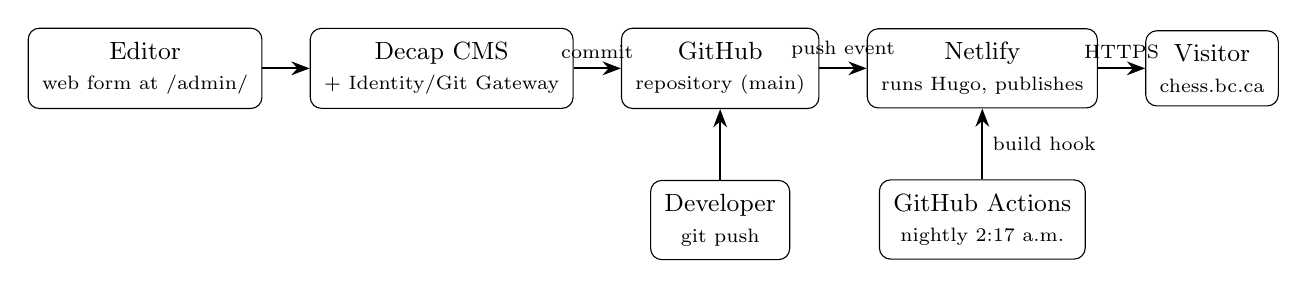
\begin{tikzpicture}[
  node distance=4mm and 6mm,
  box/.style={draw, rounded corners, align=center, inner sep=5pt,
              font=\small, minimum height=9mm},
  arr/.style={-{Stealth}, thick}
]
  \node[box] (editor) {Editor\\ \scriptsize web form at /admin/};
  \node[box, right=of editor] (decap) {Decap CMS\\ \scriptsize + Identity/Git Gateway};
  \node[box, right=of decap] (github) {GitHub\\ \scriptsize repository (main)};
  \node[box, right=of github] (netlify) {Netlify\\ \scriptsize runs Hugo, publishes};
  \node[box, right=of netlify] (visitor) {Visitor\\ \scriptsize chess.bc.ca};

  \draw[arr] (editor) -- (decap);
  \draw[arr] (decap) -- node[above, font=\scriptsize]{commit} (github);
  \draw[arr] (github) -- node[above, font=\scriptsize]{push event} (netlify);
  \draw[arr] (netlify) -- node[above, font=\scriptsize]{HTTPS} (visitor);

  \node[box, below=9mm of github] (dev) {Developer\\ \scriptsize git push};
  \draw[arr] (dev) -- (github);

  \node[box, below=9mm of netlify] (cron) {GitHub Actions\\ \scriptsize nightly 2:17 a.m.};
  \draw[arr] (cron) -- node[right, font=\scriptsize]{build hook} (netlify);
\end{tikzpicture}
\caption{Every path to the published site converges on the same pipeline:
a commit (or build trigger) causes Netlify to run Hugo and publish.}
\label{fig:flow}
\end{figure}

\textbf{An editor publishes a news item.} The editor logs into
\texttt{/admin/}, clicks \emph{News} $\rightarrow$ \emph{New News Item},
fills in the form, and clicks \emph{Publish}. Decap (via Git Gateway)
commits a new Markdown file to \texttt{content/news/} on GitHub. Netlify
notices the push, runs Hugo, and publishes the updated site. The item
appears on the home page within a minute or two, and will move itself to
the News Archive after its expiry date.

\textbf{A developer changes a template.} The developer edits files locally,
previews with \texttt{hugo server}, commits, and pushes to \texttt{main}.
The same Netlify pipeline builds and publishes. If the build fails, the
previous version keeps serving and the deploy log (Netlify dashboard
$\rightarrow$ \emph{Deploys}) shows the error.

\textbf{Nothing happens all day.} At 2:17\,a.m.\ the GitHub Actions
workflow pings the build hook; Netlify rebuilds the unchanged repository.
Any news items whose expiry date has passed drop off the home page, and the
banners reshuffle.

\section{Repository Tour}
\label{sec:repo}

\begin{table}[h]
\centering
\small
\begin{tabular}{@{}ll@{}}
\toprule
\textbf{Path} & \textbf{Contents} \\
\midrule
\texttt{content/news/} & one Markdown file per news item \\
\texttt{content/clubs/} & one file per club (grouped by city on the page) \\
\texttt{content/instruction/} & one file per instructor/academy listing \\
\texttt{content/bulletins/} & one file per bulletin issue (metadata only) \\
\texttt{content/*.md} & standalone pages (About, Membership, \ldots) \\
\texttt{data/*.yaml} & list data: arbiters, links, champions, banners, \\
 & \quad repeating events \\
\texttt{layouts/} & Hugo HTML templates and partials \\
\texttt{static/css/style.css} & the hand-written responsive stylesheet \\
\texttt{static/admin/} & Decap CMS: \texttt{index.html}, \texttt{config.yml}, \\
 & \quad the vendored \texttt{decap-cms.js} \\
\texttt{static/bulletins/} & all bulletin PDFs \\
\texttt{static/images/uploads/} & images uploaded through the CMS \\
\texttt{static/files/}, \texttt{static/AGM/}, \ldots & documents carried over from the old site \\
\texttt{hugo.toml} & Hugo configuration and navigation menus \\
\texttt{netlify.toml} & build command, Hugo version, all redirects \\
\texttt{.github/workflows/} & the nightly rebuild workflow \\
\texttt{docs/} & this report \\
\bottomrule
\end{tabular}
\caption{Repository layout.}
\label{tab:repo}
\end{table}

Two details of the content model are worth knowing before editing files by
hand:

\begin{itemize}
  \item Every file in a folder collection (news, clubs, instruction,
  bulletins) carries a hidden front-matter field \texttt{type} equal to its
  section name. The CMS uses it to keep Hugo's section index files out of
  the editors' entry lists. \emph{Keep this field} when creating files
  manually.
  \item News expiry: if \texttt{expiry\_date} is absent, templates fall
  back to the posting date plus 14 days. The CMS fills the field
  automatically at save time when an editor leaves it blank.
\end{itemize}

\section{Routine Maintenance}
\label{sec:ops}

\subsection{Inviting or removing editors}

Netlify dashboard $\rightarrow$ project \texttt{chess-bc-ca} $\rightarrow$
\emph{Identity} $\rightarrow$ \emph{Invite users}. The invitee receives an
email, sets a password, and can immediately edit at \texttt{/admin/}. To
revoke access, delete the user from the same screen. Registration is set to
invite-only; do not change this, or anyone on the internet could sign
themselves up as an editor.

\subsection{Local development}

\begin{enumerate}[nosep]
  \item Clone the repository and install Hugo (extended edition).
  \item Run \texttt{hugo server} and browse the printed local address.
        Edits to files rebuild the preview instantly.
  \item To try the CMS locally without logging in, additionally run
        \texttt{npx decap-server} and open \texttt{/admin/} on the local
        site. (This works because \texttt{config.yml} sets
        \texttt{local\_backend:\ true}, which has no effect in production.)
  \item Before pushing, run a full \texttt{hugo} build to catch errors that
        the development server can mask.
\end{enumerate}

\subsection{Upgrading the pinned versions}

\begin{itemize}
  \item \textbf{Hugo}: change \texttt{HUGO\_VERSION} in
        \texttt{netlify.toml}, test locally with the same version, push.
  \item \textbf{Decap CMS}: download a newer
        \texttt{dist/decap-cms.js} from the Decap releases and replace
        \texttt{static/admin/decap-cms.js}. Do this deliberately and test
        the admin afterwards; the file is pinned precisely so the CMS
        cannot change underneath the editors.
\end{itemize}

\subsection{DNS, domain, and certificate}

The domain registration renews yearly at the registrar --- this is the
site's only recurring cost. The registrar delegates to Netlify DNS
(nameservers \texttt{dns1--dns4.p05.nsone.net}); DNS records, should any
ever be needed (for example MX records if the Federation adopted
\texttt{@chess.bc.ca} email), are managed in the Netlify dashboard under
\emph{Domains}. The HTTPS certificate renews itself; no action is ever
required.

\subsection{Costs}

\begin{itemize}[nosep]
  \item Hosting, builds, DNS, HTTPS, editor logins: \$0 on Netlify's free
        tier. The site's traffic and build volume sit far below the free
        allowances.
  \item Domain registration: the usual yearly fee at the registrar.
  \item GitHub: free for public repositories.
\end{itemize}

\section{Troubleshooting}
\label{sec:trouble}

\begin{description}
  \item[An editor's form comes up blank, or the admin misbehaves.] Have
  them hard-refresh the browser (Ctrl+Shift+R) to shed a stale cached copy
  of the CMS, and if that fails, log out and back in (a stale login token
  produces exactly this symptom).

  \item[A change was published but the site did not update.] Check the
  Netlify dashboard $\rightarrow$ \emph{Deploys}. A red ``Failed'' deploy
  means the build broke; open it to read the Hugo error. The site keeps
  serving the last good version meanwhile.

  \item[Expired news is not moving to the archive.] The nightly rebuild has
  probably stopped. Check the repository's \emph{Actions} tab on GitHub:
  the ``Nightly Netlify rebuild'' workflow should show nightly runs. Note
  that GitHub automatically pauses scheduled workflows in repositories with
  no commits for 60 days (it emails a warning first); any push, or pressing
  \emph{Run workflow}, resumes it. Also confirm the
  \texttt{NETLIFY\_BUILD\_HOOK} secret still matches a valid build hook in
  Netlify.

  \item[Something was deleted or broken by mistake.] Nothing is lost. Find
  the offending commit in the repository history on GitHub and revert it,
  or restore the previous version of the file. The next push republishes
  the corrected site. Netlify's \emph{Deploys} list also allows one-click
  ``publish deploy'' rollback to any earlier build.

  \item[A mangled entry breaks the layout below it.] The site allows raw
  HTML inside content (editors' rich text needs it), so an unterminated tag
  pasted into an entry can visually swallow what follows. Edit the entry
  and remove the stray fragment. This occurred once during migration
  (a dangling \texttt{</p} in a club listing inherited from the old site).
\end{description}

\section{Key Reference}
\label{sec:ref}

\begin{table}[h]
\centering
\small
\begin{tabular}{@{}ll@{}}
\toprule
Live site & \url{https://chess.bc.ca} \\
Editing interface & \url{https://chess.bc.ca/admin/} \\
Repository & \url{https://github.com/stmorgan/chess.bc.ca-hugo} \\
Netlify project & \texttt{chess-bc-ca} (dashboard: app.netlify.com) \\
Hugo version & 0.163.3 extended (pinned in \texttt{netlify.toml}) \\
Decap CMS version & 3.14.1 (vendored at \texttt{static/admin/decap-cms.js}) \\
Nightly rebuild & GitHub Actions, 10:17 UTC (2:17\,a.m.\ Pacific) \\
Nameservers & \texttt{dns1.p05.nsone.net} \ldots{} \texttt{dns4.p05.nsone.net} \\
Content at migration & 99 news items, 45 clubs, 11 instruction listings, \\
 & \quad 485 bulletins, 234 champions entries \\
Migration completed & July 8, 2026 (DNS cutover) \\
\bottomrule
\end{tabular}
\caption{Quick reference.}
\label{tab:ref}
\end{table}

\end{document}
